\chapter{DESARROLLO DEL PROYECTO}

En este capítulo se describe el proceso de desarrollo del proyecto SISTAL, abordando la construcción de una solución funcional basada en la arquitectura y tecnologías definidas previamente. El desarrollo se enfocó en la implementación del módulo de funcionarios, validando la viabilidad técnica de la propuesta de reingeniería.

%------------------------------------------------------------------------

\section{Stack tecnológico utilizado}

Haremos un repaso por las tecnologías definidas para realizar este proyecto, argumentando cada una de las decisiones e indicando los frameworks y todos los detalles respectivos.

\subsection{Tecnologías de frontend}

\subsubsection{React}

React fue elegido como tecnología de frontend debido a su arquitectura\footnote{Arquitectura aquí hace referencia al patrón de diseño y organización de los archivos o componentes de código.} basada en componentes, la cual permite construir interfaces desacopladas, reutilizables y fácilmente mantenibles. Esta característica resulta fundamental en aplicaciones donde existen múltiples vistas y flujos de usuario diferenciados, como es el caso de SISTAL.

Desde un punto de vista técnico, React facilita:

\begin{itemize}
    \item La separación clara entre lógica de presentación y lógica de negocio.
    \item El consumo eficiente de APIs REST.
    \item La escalabilidad del frontend sin afectar el backend.
\end{itemize}

Su adopción permite superar una de las principales limitaciones del sistema legacy, donde la interfaz y la lógica de negocio se encontraban fuertemente acopladas.

\subsubsection{Tailwind CSS}

Tailwind CSS fue seleccionado como framework de estilos debido a su enfoque utility-first, el cual permite construir interfaces consistentes sin necesidad de escribir grandes cantidades de CSS personalizado y alineándose muy bien con la arquitectura de componentes de React.

Las razones técnicas de su elección incluyen:

\begin{itemize}
    \item Reducción del acoplamiento entre estilos y componentes.
    \item Mayor velocidad de desarrollo y menor complejidad en el mantenimiento.
\end{itemize}

En el contexto de SISTAL, Tailwind facilita la rápida implementación de interfaces alineadas con los prototipos definidos, manteniendo un diseño coherente y controlado.

\subsection{Tecnologías de backend}

\subsubsection{Go}

Go fue seleccionado como lenguaje de backend por su eficiencia, simplicidad y orientación al desarrollo de servicios.

Las razones técnicas principales son:

\begin{itemize}
    \item Lenguaje compilado y tipado, que reduce errores en tiempo de ejecución.
    \item Alto rendimiento y bajo consumo de recursos.
    \item Excelente manejo de concurrencia mediante goroutines.
\end{itemize}

Estas características lo hacen especialmente adecuado para arquitecturas basadas en microservicios y despliegues contenerizados, como los propuestos en SISTAL.

\subsubsection{Gin}

Gin se utiliza como framework HTTP debido a su ligereza y alto rendimiento.

Su elección se justifica porque:

\begin{itemize}
    \item Proporciona un routing eficiente y claro.
    \item Introduce un mínimo de abstracciones, manteniendo control sobre la lógica.
    \item Facilita la construcción de APIs REST bien definidas.
\end{itemize}

Gin permite desarrollar servicios backend simples, rápidos y fáciles de mantener, alineados con la filosofía de Go.

\subsubsection{GORM}

GORM fue seleccionado como ORM para Go debido a su madurez y facilidad de integración con PostgreSQL.

Desde el punto de vista técnico:

\begin{itemize}
    \item Simplifica el acceso a datos mediante abstracción del SQL.
    \item Reduce errores comunes en consultas manuales.
    \item Facilita el mapeo entre modelos de dominio y tablas relacionales.
\end{itemize}

Su uso mejora la mantenibilidad del código y favorece la coherencia entre el modelo de datos y la lógica de negocio.

% \subsubsection{Arquitectura hexagonal}
% 
% La arquitectura hexagonal fue adoptada con el objetivo de desacoplar la lógica de negocio de los detalles de infraestructura.
% 
% Las razones técnicas incluyen:
% 
% - Separación clara entre dominio, aplicación e infraestructura.
% 
% - Facilidad para cambiar tecnologías sin afectar el núcleo del sistema.
% 
% - Mejora significativa en testabilidad y mantenibilidad.
% 
% En SISTAL, esta arquitectura permite que el dominio del negocio se mantenga independiente del framework, la base de datos o el mecanismo de comunicación, alineándose con los principios de diseño limpio.

\subsection{Persistencia de datos}

\subsubsection{PostgreSQL}

PostgreSQL fue elegido como sistema gestor de base de datos por su robustez, confiabilidad y cumplimiento de estándares ACID.

Las razones técnicas incluyen:

\begin{itemize}
    \item Soporte completo para integridad referencial.
    \item Manejo eficiente de transacciones.
    \item Alta estabilidad en entornos productivos.
\end{itemize}

Esta elección permite resolver las deficiencias estructurales del sistema legacy, garantizando consistencia y trazabilidad de la información.

\subsection{Infraestructura y DevOps}

\subsubsection{Docker}

Docker se utiliza para contenerizar los distintos componentes del sistema.

Desde el punto de vista técnico:

\begin{itemize}
    \item Garantiza consistencia entre entornos.
    \item Reduce errores de despliegue.
    \item Facilita la portabilidad de los servicios.
\end{itemize}

Docker es un pilar fundamental para una arquitectura cloud-native.

\subsubsection{Kubernetes}

Kubernetes se emplea como plataforma de orquestación de contenedores.

Su elección se justifica por:

\begin{itemize}
    \item Escalabilidad automática de servicios.
    \item Alta disponibilidad.
    \item Gestión centralizada del ciclo de vida de aplicaciones.
\end{itemize}

Kubernetes permite operar el sistema de forma robusta y preparada para crecimiento futuro.

\subsubsection{Google Cloud Platform}

GCP fue seleccionada como plataforma cloud por su integración nativa con Kubernetes y su enfoque en servicios administrados.

Las razones técnicas incluyen:

\begin{itemize}
    \item Google Kubernetes Engine (GKE) como servicio gestionado.
    \item Infraestructura altamente disponible.
    \item Reducción de carga operativa.
\end{itemize}

GCP permite desplegar SISTAL en un entorno real de producción, validando la arquitectura propuesta.

\subsubsection{GitHub Actions}

GitHub Actions se utiliza como herramienta de integración y despliegue continuo.

Técnicamente aporta:

\begin{itemize}
    \item Automatización del ciclo de desarrollo.
    \item Integración nativa con GitHub.
    \item Despliegues repetibles y controlados.
\end{itemize}

Su adopción asegura calidad, trazabilidad y eficiencia en el proceso de entrega de software.


\section{Gestión del proyecto y trabajo colaborativo}

La siguiente sección explica como se utilizó la metodología de trabajo seleccionada y como se organizó el trabajo del proyecto.

\subsection{Metodología de Trabajo}

La metodología seleccionada para la etapa de desarrollo del proyecto fue \textit{Scrum}, por tratarse de un marco de trabajo ágil orientado a la gestión incremental del software, que promueve la adaptación al cambio, la entrega continua de valor y una comunicación constante entre los integrantes del equipo, además de alinearse muy bien con las metodologías DevOps.

El desarrollo se estructuró en un ciclo de tres semanas, organizado en iteraciones cortas en las que se planificaron, implementaron y revisaron funcionalidades priorizadas. Este enfoque facilitó el seguimiento del avance, la detección temprana de problemas y la incorporación de mejoras de manera progresiva, alineando el resultado final con los objetivos planteados desde el inicio del proyecto.

Como herramienta de gestión de proyectos se utilizó \textbf{GitHub Projects}, ya que se integra directamente con los repositorios y el flujo de trabajo basado en ramas que se mencionan a continuación, centralizando las tareas asignadas y la revisión de código.

\subsection{Flujo de Trabajo con Git}

Como herramienta de control de versiones de los microservicios se utilizó el clásico \textbf{Git} y para complementar con un flujo de desarrollo organizado y alineado a prácticas DevOps se utilizó un modelo adaptado de \textbf{\textit{GitFlow}} con las siguientes características:

\begin{itemize}
    \item Rama principal \textit{\textbf{Main}} donde está la versión estable de cada microservicio y la cual estará en uso por los clientes.
    \item Rama \textbf{\textit{QA}} donde se aloja una nueva versión del microservicio que se encuentra en entorno de pruebas para pronto ser integrada en \textit{Main}
    \item Rama \textbf{\textit{Develop}} donde se encuentra la última versión con los cambios realizados por el equipo de desarrollo, si se decide lanzar esta versión se integra a la rama QA para que sea probada en un entorno de preparación.
    \item Rama \textbf{\textit{Feature}} donde se implementa una nueva tarea acordada en la planificación. Esta rama primero se copia de \textit{Develop} para trabajar sin alterar el trabajo ya realizado y al finalizarse se vuelve a integrar a \textit{Develop} donde los desarrolladores deben aprobar su validación antes.
\end{itemize}

% Ejemplo del uso de esta metodología

\subsection{Organización en GitHub}

Siguiendo los diagramas de arquitectura y despliegue previamente expuestos de la \autoref{fig:diagrama-arquitectura} y \autoref{fig:diagrama-despliegue}, se creó un repositorio por microservicio, cada uno siguiendo una plantilla de despliegue que permitira al comenzar el desarrollo que cada versión nueva se pueda testear inmediatamente en un servidor de pruebas.

% poner fotos del repositorio

\section{Diseño de Interfaz de Usuario}

En esta sección se presentan los diseños de la nueva interfaz de usuario destinada a los funcionarios del sistema. Esta introduce una serie de mejoras orientadas a optimizar la usabilidad, accesibilidad y coherencia visual del sistema, entre las cuales destacan las siguientes:

\begin{itemize}
    \item \textbf{Estandarización de paneles de control}: se adopta un diseño más estandarizado en los paneles de control, alineado con patrones de diseño ampliamente utilizados en aplicaciones modernas. Esto facilita la comprensión de la información presentada, reduce la curva de aprendizaje y genera una experiencia más familiar e intuitiva para los usuarios.

    \item \textbf{Diseño adaptativo (responsive)}: la interfaz fue concebida bajo principios de diseño adaptativo, permitiendo su correcta visualización y funcionamiento en distintas resoluciones y tamaños de pantalla. Esto garantiza una experiencia consistente tanto en equipos de escritorio como en dispositivos portátiles.

    \item \textbf{Mayor consistencia visual}: el uso homogéneo de colores, tipografías y componentes gráficos contribuye a una identidad visual coherente, fortaleciendo la percepción de profesionalismo y facilitando la navegación entre las distintas secciones del sistema.
\end{itemize}

Las interfaces fueron diseñadas utilizando la herramienta \textbf{Figma}, lo que permitió prototipar y validar visualmente la experiencia de usuario antes de su implementación. Con el objetivo de mejorar la legibilidad y visualización de los elementos, algunas de las figuras se presentan en formato horizontal.

\begin{sidewaysfigure}
    \centering
    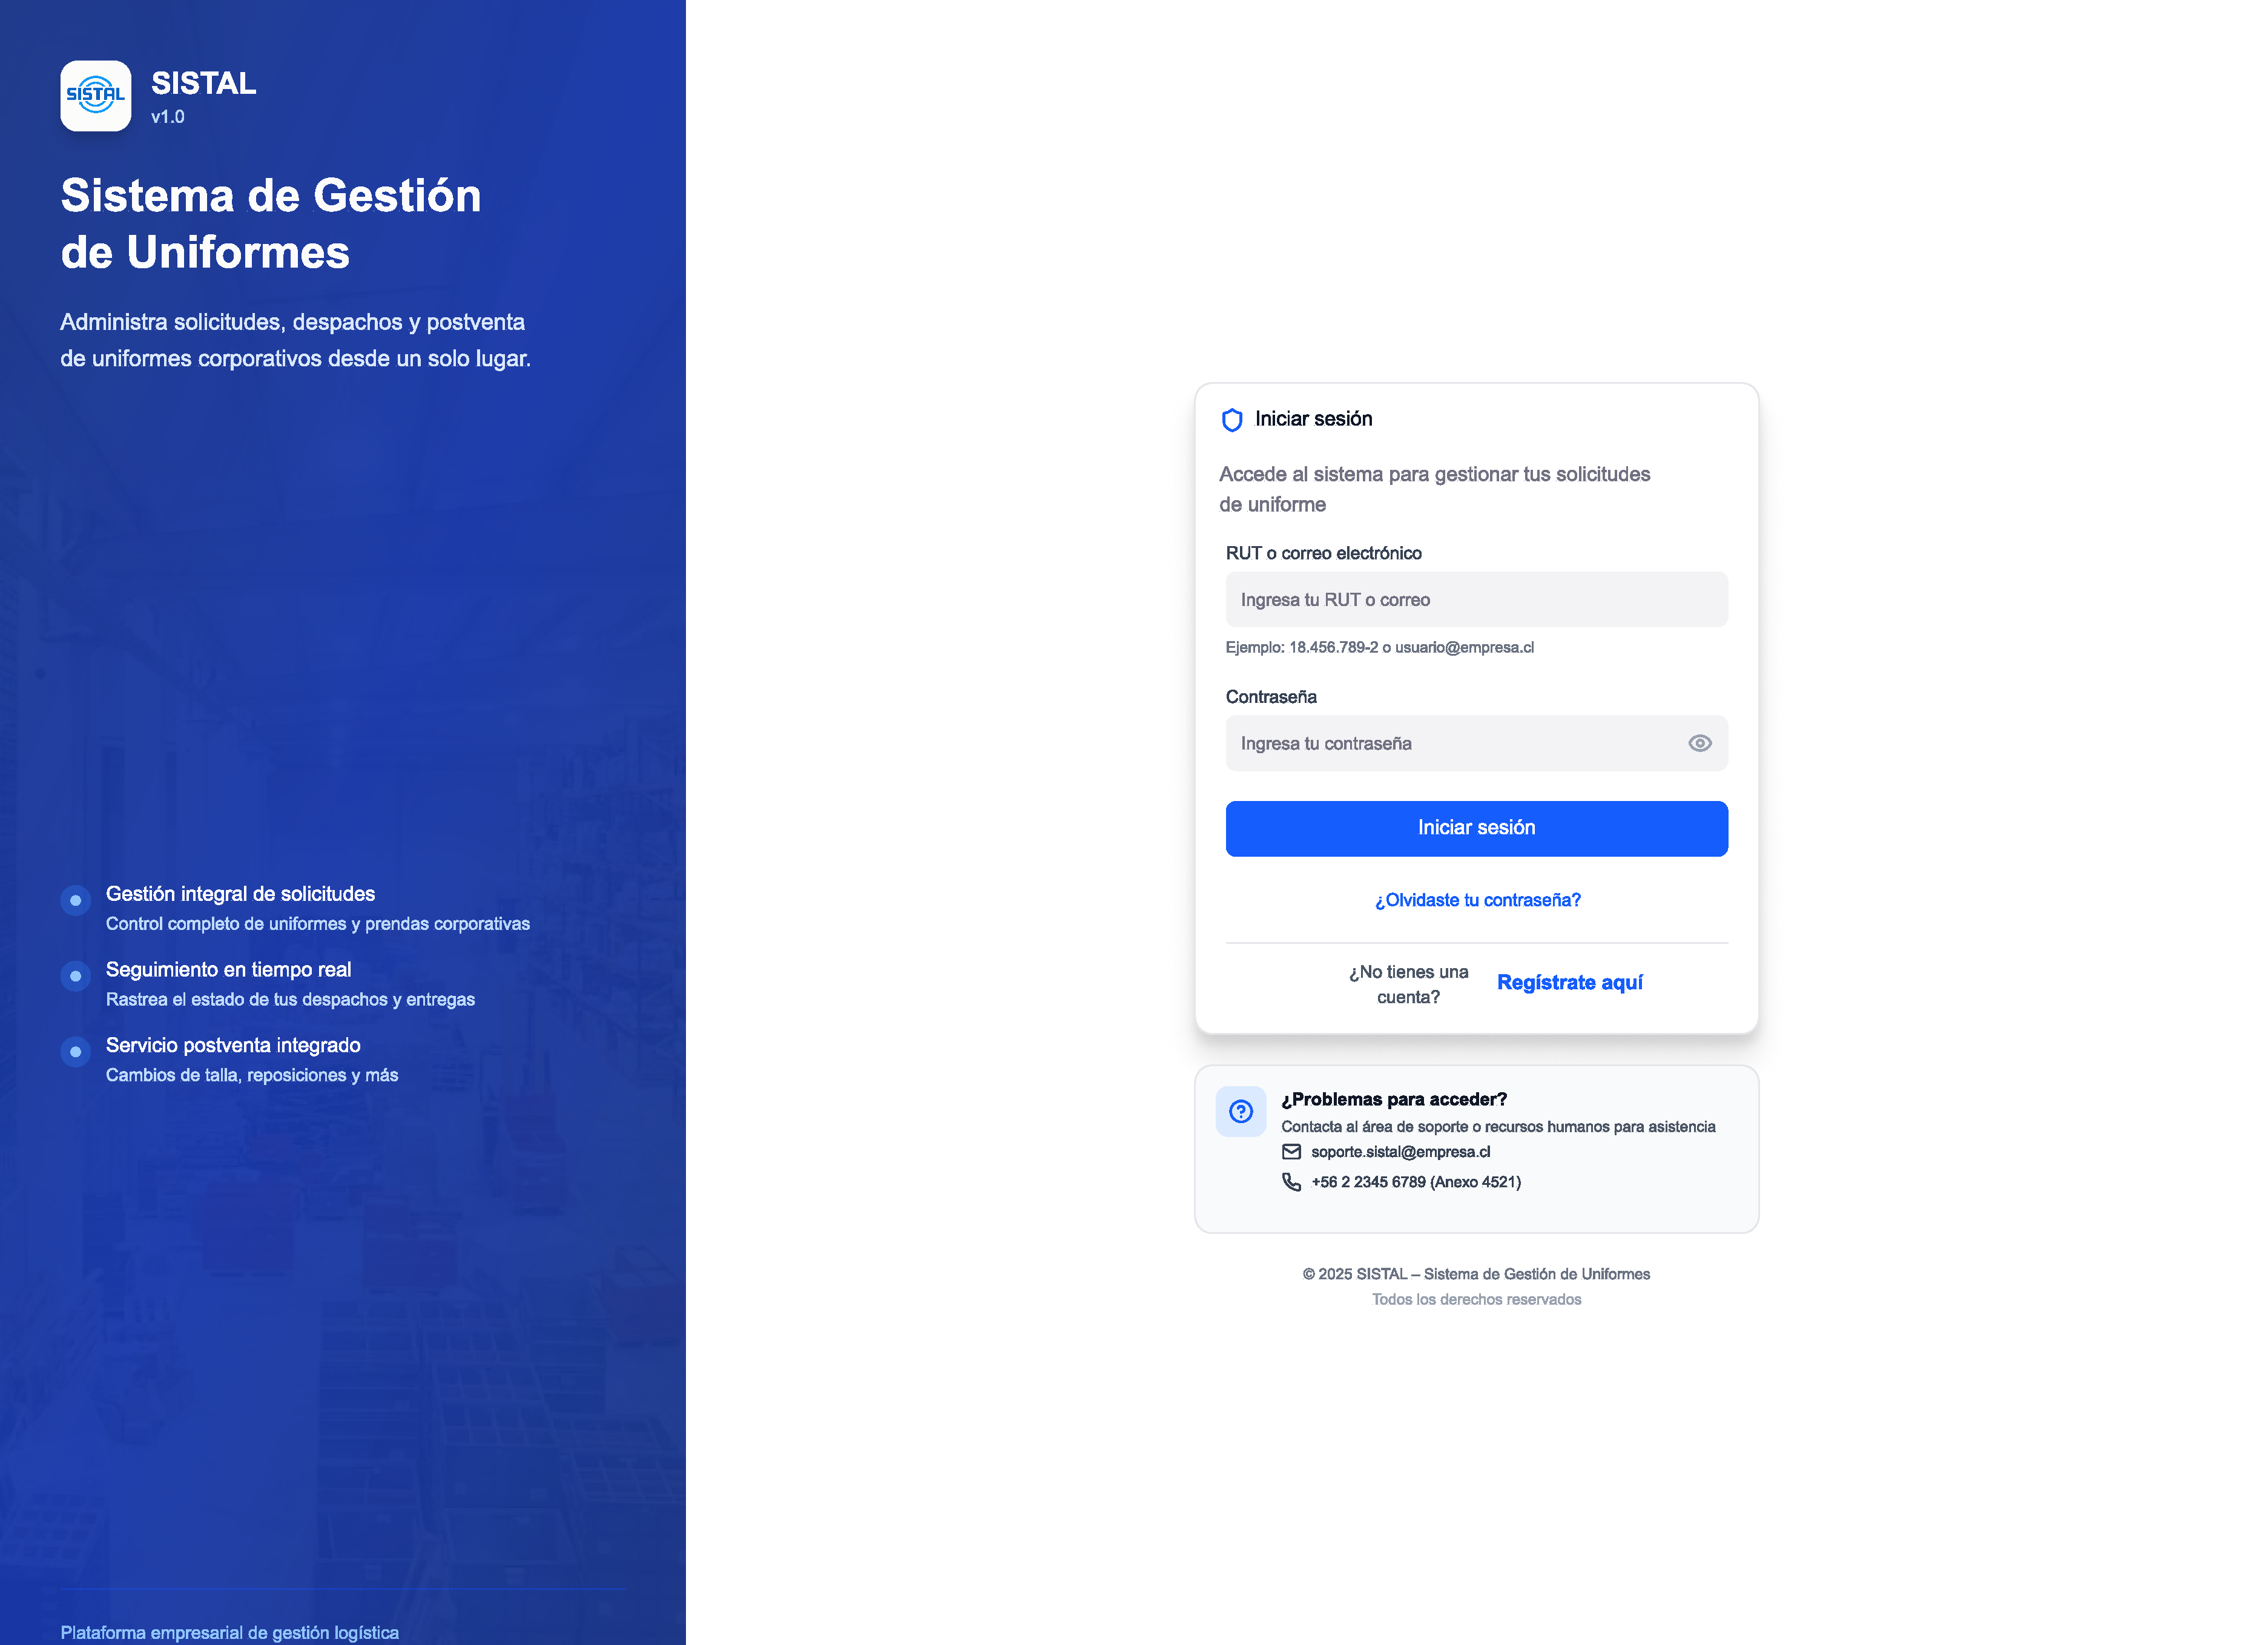
\includegraphics[width=0.9\textwidth, frame]{figuras/figma/Inicio de sesión.pdf}
    \caption{GUI de inicio de sesión} \label{fig:figma-login}
    \sourcefig{Elaboración Propia en Figma}{}{}
\end{sidewaysfigure}
\newpage

\begin{sidewaysfigure}
    \centering
    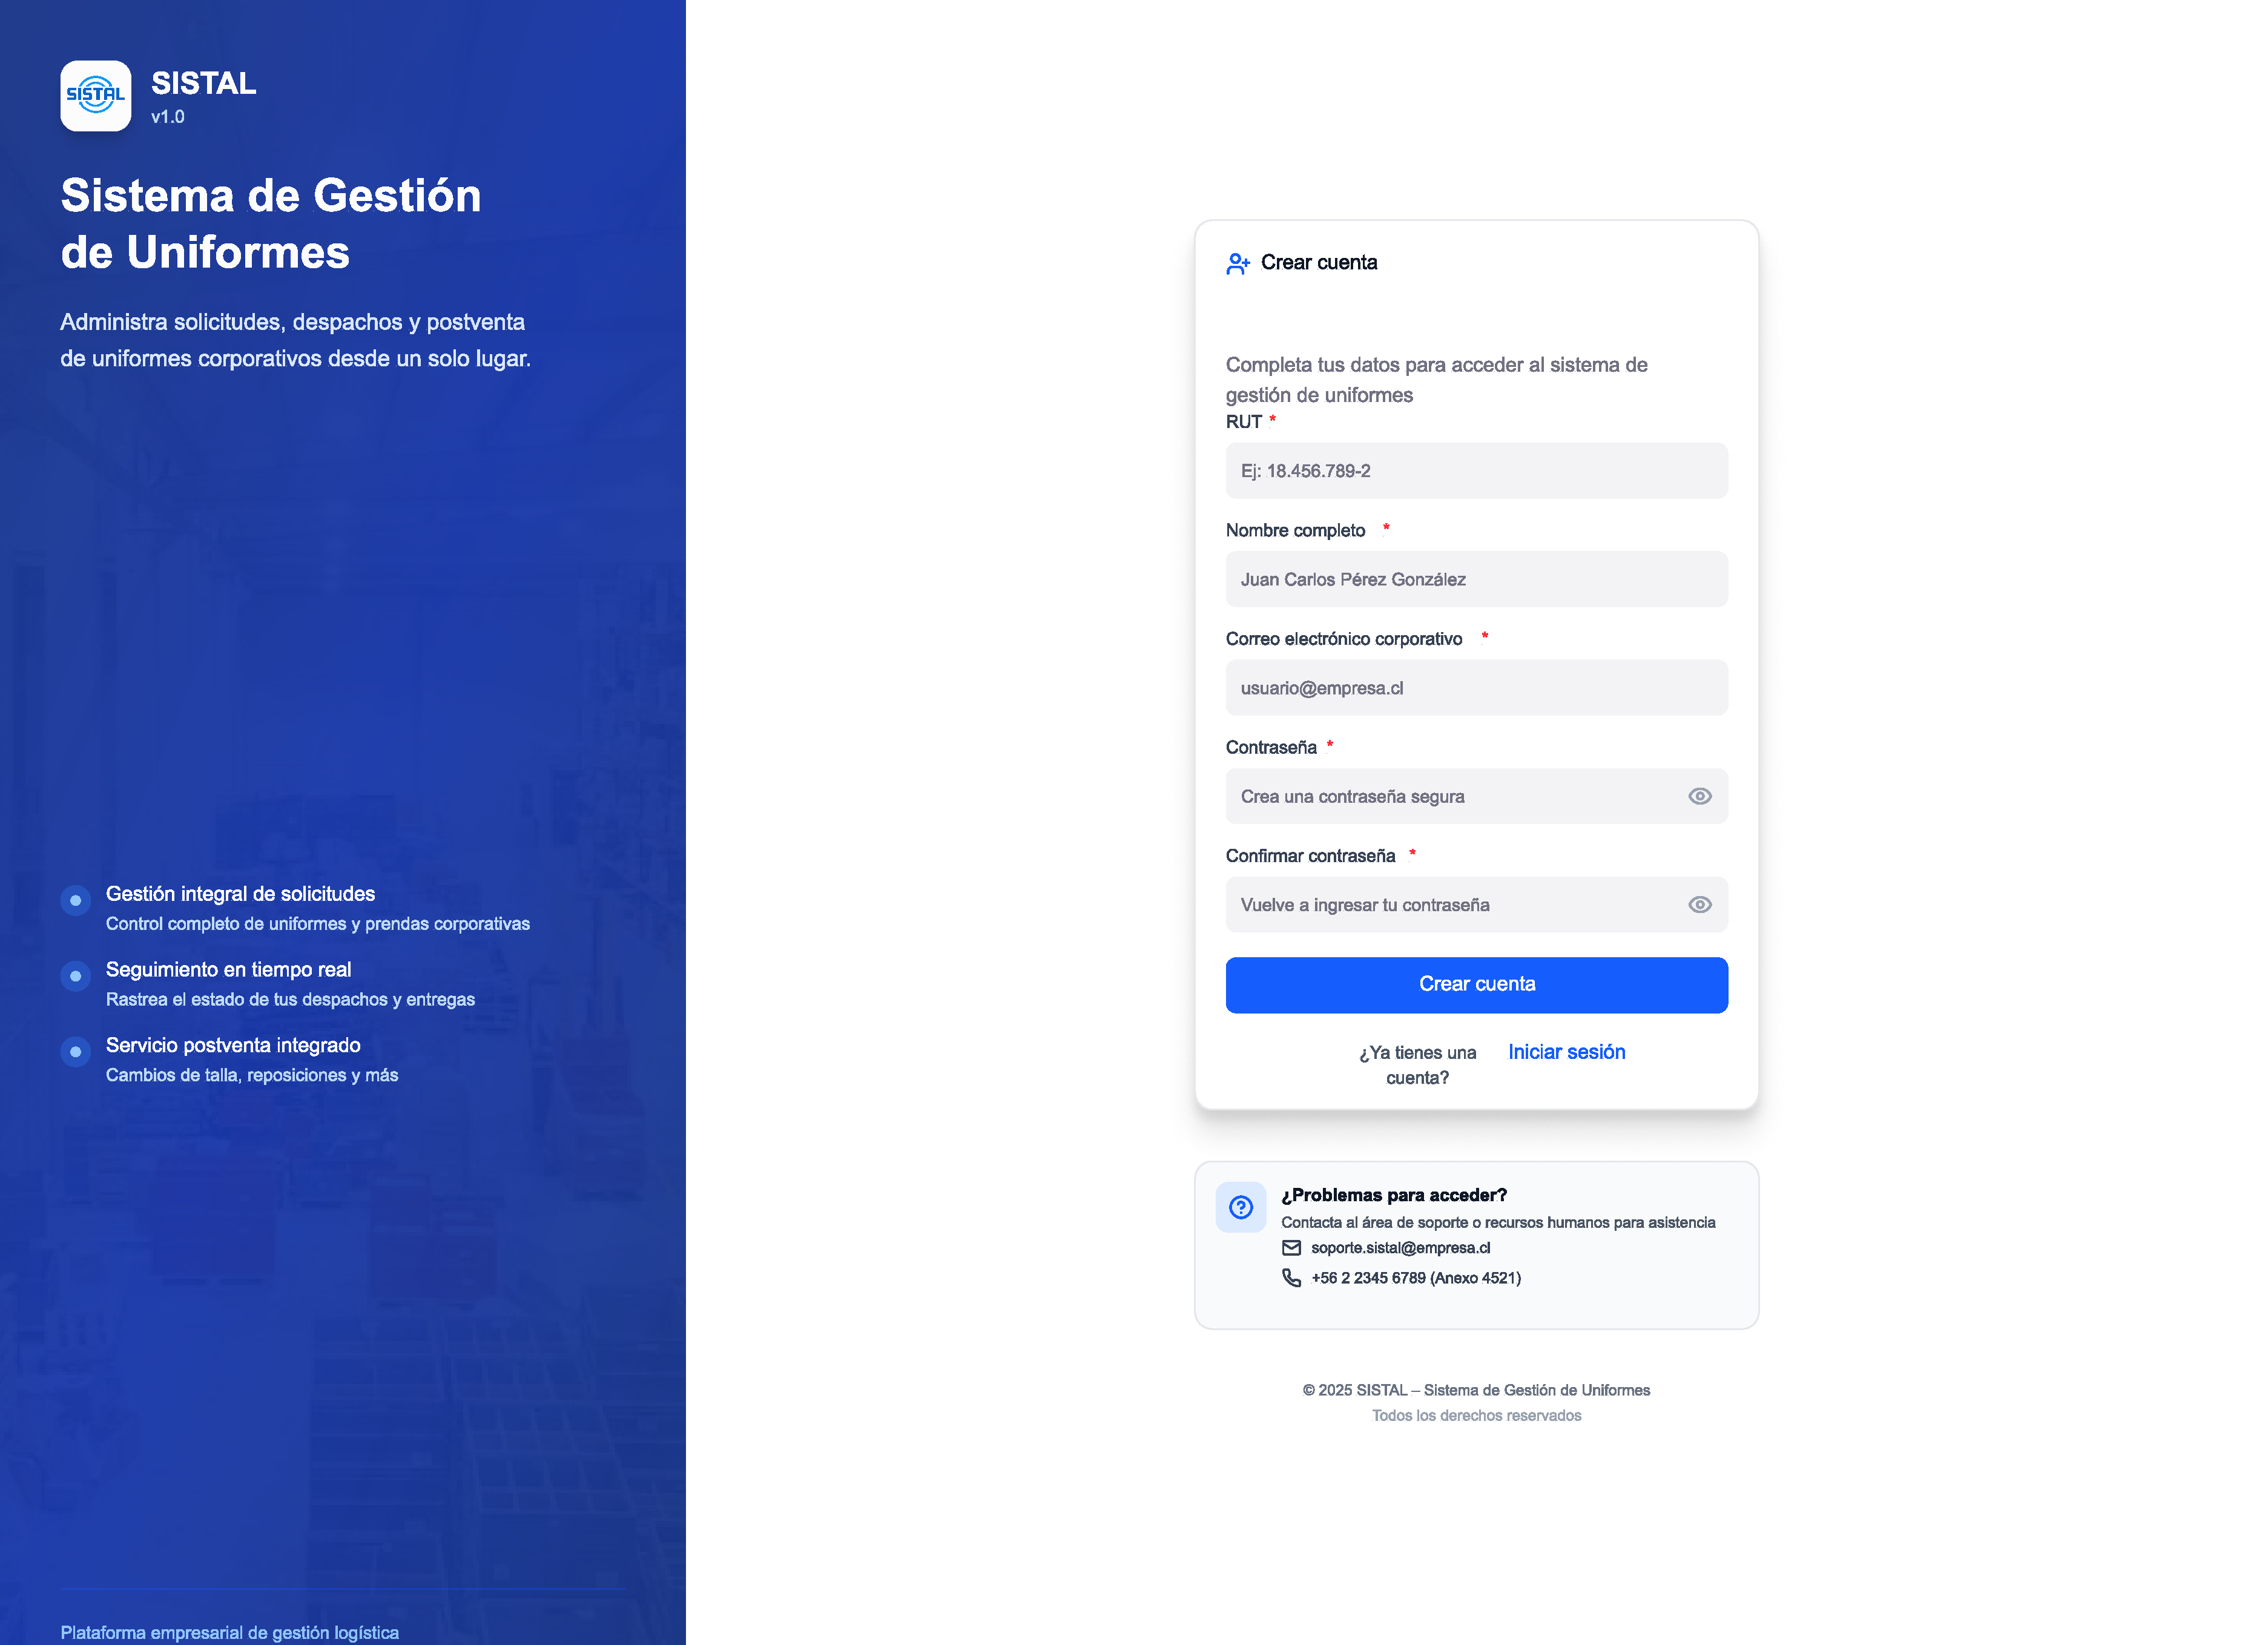
\includegraphics[width=0.9\textwidth, frame]{figuras/figma/Registro.pdf}
    \caption{GUI de registro de usuario} \label{fig:figma-registro}
    \sourcefig{Elaboración Propia en Figma}{}{}
\end{sidewaysfigure}
\newpage

\begin{figure}[p]
    \centering
    \includegraphics[width=\linewidth, frame]{figuras/figma/Wireframe Mis Solicitudes.pdf}
    \caption{GUI Panel principal de Funcionario} \label{fig:figma-funcionario}
    \sourcefig{Elaboración Propia en Figma}{}{}
\end{figure}

\begin{figure}[p]
    \centering
    \includegraphics[width=0.8\linewidth]{figuras/figma/Notificaciones.pdf}
    \caption{GUI Botón de notificaciones} \label{fig:figma-notificaciones}
    \sourcefig{Elaboración Propia en Figma}{}{}
\end{figure}

\begin{sidewaysfigure}
    \centering
    \includegraphics[width=\textheight, frame]{figuras/figma/Mis Solicitudes.pdf}
    \caption{GUI solicitudes realizadas por el funcionario} \label{fig:figma-solicitudes}
    \sourcefig{Elaboración Propia en Figma}{}{}
\end{sidewaysfigure}

\begin{figure}[p]
    \centering
    \includegraphics[height=0.93\textheight, frame]{figuras/figma/Solicitud cambio de sucursal.pdf}
    \caption{GUI de solicitud de cambio de sucursal} \label{fig:figma-cambio-sucursal}
    \sourcefig{Elaboración Propia en Figma}{}{}
\end{figure}

\begin{figure}[p]
    \centering
    \includegraphics[width=\linewidth, frame]{figuras/figma/Solicitud cambio de talla.pdf}
    \caption{GUI de solicitud de cambio de talla} \label{fig:figma-cambio-talla}
    \sourcefig{Elaboración Propia en Figma}{}{}
\end{figure}

\begin{sidewaysfigure}
    \centering
    \includegraphics[width=\textheight, frame]{figuras/figma/Seguimiento del despacho.pdf}
    \caption{GUI de seguimiento de despachos} \label{fig:figma-despachos}
    \sourcefig{Elaboración Propia en Figma}{}{}
\end{sidewaysfigure}

\begin{figure}[p]
    \centering
    \includegraphics[height=0.93\textheight, frame]{figuras/figma/Mi Cuenta.pdf}
    \caption{GUI de información de cuenta funcionario} \label{fig:figma-cuenta}
    \sourcefig{Elaboración Propia en Figma}{}{}
\end{figure}
